% --------------------------------------------------------------
% This is all preamble stuff that you don't have to worry about.
% Head down to where it says "Start here"
% --------------------------------------------------------------
 
\documentclass[12pt]{article}
 
\usepackage[margin=1in]{geometry} 
\usepackage{amsmath,amsthm,amssymb}
\usepackage{gensymb}
\usepackage{graphicx}
 \usepackage{tikz,pgfplots}
\usepackage{float}
\usepackage{tikz}
\usepackage{enumitem}

\newcommand{\N}{\mathbb{N}}
\newcommand{\Z}{\mathbb{Z}}

\newcommand{\slantedgrid}[4]{%
   \pgfmathtruncatemacro{\result}{#1+#3}
   \foreach \x in {#1,...,\result} \draw (\x,#2) -- ++(#4,#4);%
   \pgfmathtruncatemacro{\result}{#2+#4}
   \foreach \y in {#2,...,\result} \draw (#1+\y-#2,\y) -- ++(#3,0);%
 }
 
\newenvironment{theorem}[2][Theorem]{\begin{trivlist}
\item[\hskip \labelsep {\bfseries #1}\hskip \labelsep {\bfseries #2.}]}{\end{trivlist}}
\newenvironment{lemma}[2][Lemma]{\begin{trivlist}
\item[\hskip \labelsep {\bfseries #1}\hskip \labelsep {\bfseries #2.}]}{\end{trivlist}}
\newenvironment{exercise}[2][Exercise]{\begin{trivlist}
\item[\hskip \labelsep {\bfseries #1}\hskip \labelsep {\bfseries #2.}]}{\end{trivlist}}
\newenvironment{problem}[2][Problem]{\begin{trivlist}
\item[\hskip \labelsep {\bfseries #1}\hskip \labelsep {\bfseries #2.}]}{\end{trivlist}}
\newenvironment{question}[2][Question]{\begin{trivlist}
\item[\hskip \labelsep {\bfseries #1}\hskip \labelsep {\bfseries #2.}]}{\end{trivlist}}
\newenvironment{corollary}[2][Corollary]{\begin{trivlist}
\item[\hskip \labelsep {\bfseries #1}\hskip \labelsep {\bfseries #2.}]}{\end{trivlist}}
 
\begin{document}
\providecommand{\e}[1]{\ensuremath{\times 10^{#1}}}
% --------------------------------------------------------------
%                         Start here
% --------------------------------------------------------------
 
\title{HW 3}%replace X with the appropriate number
\author{Levon Dovlatyan, SI: 24451582\\ %replace with your name
E45} %if necessary, replace with your course title
 
\maketitle
 
\begin{problem}{3.3} %You can use theorem, exercise, problem, or question here.  Modify x.yz to be whatever number you are proving
Why is there no base-centered cubic lattice in Table 3.2? (Use a sketch to answer)
\end{problem}
 
By placing several base-centered cubics side by side and looking at cross sectional view, we can see why there is no need for a base-centered cubic. The unit cell of a base-centered cubic can be draw using the center base-centered points as will which would make it a simple tetragonal. So a base-centered cubic is infact just a tetragonal, hence there is no need for one. \\*[1cm]
 \begin{figure}[H]
 \centering
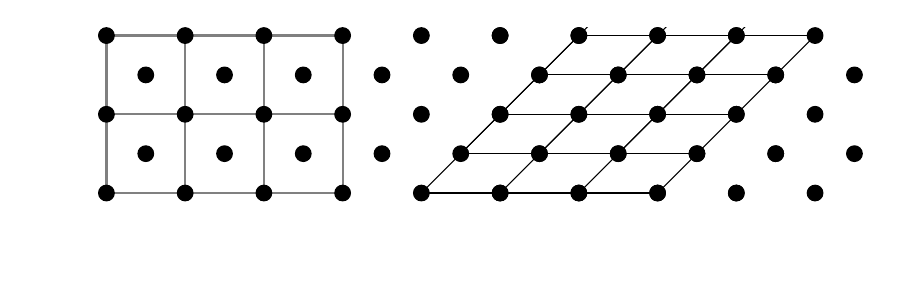
\begin{tikzpicture}
    \clip (-1,-1) rectangle (10cm,2.1cm); 
    \draw[style=help lines,thick] (0,0) grid[step=1cm] (3,2);

    \foreach \x in {0,1,...,9}
    {
        \foreach \y in {0,1,...,2}
        {
            \node[draw,circle,inner sep=2pt,fill] at (\x,\y) {};
            \node[draw,circle,inner sep=2pt,fill] at (\x+0.5,\y+0.5) {};
        }
    }
    \slantedgrid{4}{0}{3}{2}
    \slantedgrid{4.5}{0.5}{3}{2}
    \foreach \x in {0,1,...,3}
    {
        \foreach \y in {0,1,...,2}
        {
            \node[draw,circle,inner sep=2pt,fill] at (\x+5,\y) {};
            \node[draw,circle,inner sep=2pt,fill] at (\x+5.5,\y+0.5) {};
        }
    }
\end{tikzpicture}
\caption{A set of lattice points showing the cross-sectional view of several base-centered cubics.}
\end{figure}

\begin{problem}{3.7}
Calculate the density of Mg, an hcp metal. (Note Problem 3.11 for the ideal c.a ratio.)
\end{problem}

The volume of a hexagonal is $V = h*A$ where h is the height and A is the area of the base. The area of the base is $A = a^2 * \sin{60}$ where a is the edge length. The height of the hexagonal is related to the edge length where $h = 1.633*a$. For an hcp, $a = 2r_{Mg}$ where $r_{Mg} = 0.160$ nm.

\begin{align*}
\rho &= \frac{2 \,\text{atoms}}{h*A} = \frac{2 \,\text{atoms}}{1.633a^3\sin{60}} = \frac{2 \,\text{atoms}}{1.633\sin{60}(0.32\e{-9}\,\text{m})^3} * \frac{24.31\,\text{g}}{6.023\e{23}\, \text{atoms}} * (\frac{1\,\text{m}}{10^2\,\text{cm}})^3 \\
 &= 1.74\,\text{g}/\text{cm}^3
\end{align*}

\begin{problem}{3.10}
Calculate the APF of 0.74 for hcp metals.
\end{problem}

From the previous problem we know that the volume of an hcp unit cell is $V_{cell} = 1.633\,a^3\sin{60}$ where $a = 2r_{atom}$. The hcp structure also contains 2 full atoms inside it. Using this data we can solve for teh APF.

\begin{align*}
\text{APF} = \frac{V_{atoms}}{V_{cell}} = \frac{2*(\frac{4\pi}{3}{r_{atom}}^3)}{1.633\,\sin{60}{(2r_{atom})}^3} = \frac{2\pi}{3\sqrt{3}*1.633} = 0.74
\end{align*}

\begin{problem}{3.17}
Calculate the IPF for cristobalite (Figure 3.11).
\end{problem}

\begin{align*}
V_{atoms} &= 8(\frac{4\pi {r_{Si^{4+}}}^3}{3}) + 16(\frac{4\pi {r_{O^{2-}}}^3}{3}) = 0.156 \,{\text{nm}}^3\\
V_{cube} &= a^3 = \frac{d^3}{2^{\frac{3}{2}}} = \frac{(8r_{O^{2-}} + 2r_{Si^{4+}})^3}{2^{\frac{3}{2}}} = 0.516\, {\text{nm}}^3 \\
\text{IPF} &= \frac{V_{atoms}}{V_{cube}} = \frac{0.156}{0.516} = 0.317
\end{align*}

\begin{problem}{3.27}
\textbf{(a)} Sketch, in a cubic unit cell, a [111] and a [112] lattice direction. \textbf{(b)} Use a trigonometric calculation to determine the angle between these two directions. \textbf{(c)} Use Equation 3.3 to determine the angle between these two directions.
\end{problem}

\textbf{(a)} This was done in python,

\begin{figure}[H]
\centering
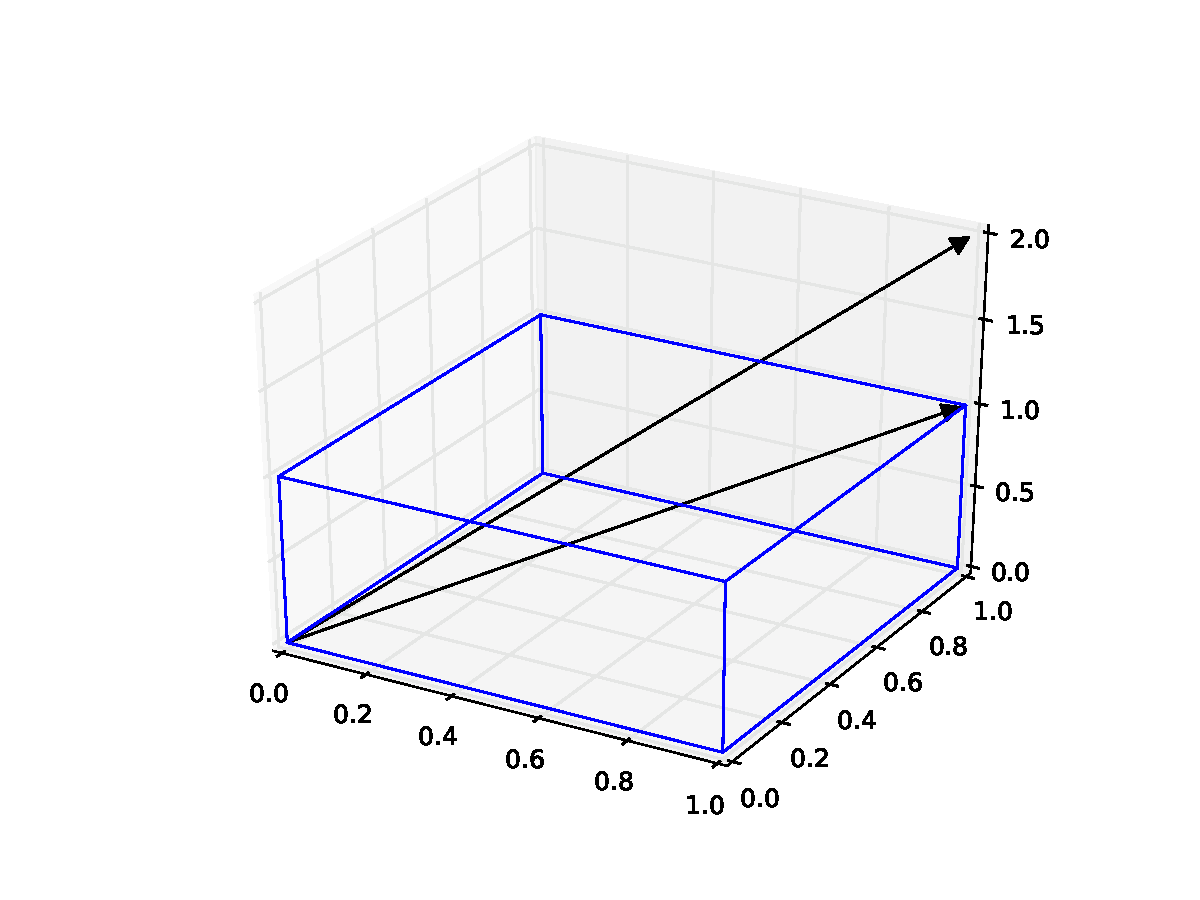
\includegraphics[width=400pt]{graph_p3_27.pdf}
\caption{cubic unit cell with vectors [111] and [112]}
\end{figure}

\textbf{(b)} Using simple geometry we get to this point, \\*[1cm]
\begin{figure}[H]
\centering
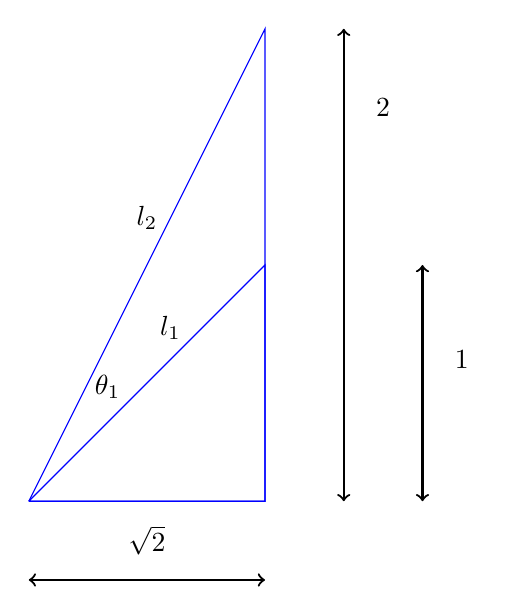
\begin{tikzpicture}
\draw [blue] (0,0) -- (3,0) -- (3,3) -- (0,0);
\draw [blue] (0,0) -- (3,0) -- (3,6) -- (0,0);
\node at (1,1.45) {\textbf{$\theta_1$}};
\draw [<->, thick, black] (4,0) -- (4,6);
\draw [<->, thick, black] (5,0) -- (5,3);
\draw [<->, thick, black] (0,-1) -- (3,-1);
\node at (1.8,2.2) {\textbf{$l_1$}};
\node at (1.5,3.6) {\textbf{$l_2$}};
\node at (1.5,-0.5) {\textbf{$\sqrt{2}$}};
\node at (5.5,1.8) {\textbf{$1$}};
\node at (4.5,5) {\textbf{$2$}};
\end{tikzpicture}
\end{figure}

Where $l_1$ represents the [111] vector and $l_2$ represents the [112] vector. Using law of cosines we see that $2^2 = {l_1}^2 + {l_2}^2 - 2l_1l_2\cos{\theta_2}$. Where $l_1 = \sqrt{3}$ and $l_2 = \sqrt{6}$. Pluggin this in, we get $\theta_1 = \arccos{\frac{4}{\sqrt{18}}} \approx 19.5$ degrees. \\

\textbf{(c)} 

\begin{align*}
V_1 = (1,1,1) ,\,\,\, V_2 = (1,1,2) \\
\cos{\theta} = \frac{V_1 \dot V_2}{|V_1||V_2|} = \frac{1*1 + 1*1 + 1*2}{\sqrt{1^2 + 1^2 + 1^2}\sqrt{1^2 + 1^2 + 2^2}} = \frac{4}{\sqrt{18}}
\end{align*}

This is the same as part b, the answer is $\theta \approx 19.5$ degrees.








% --------------------------------------------------------------
%     You don't have to mess with anything below this line.
% --------------------------------------------------------------
 
\end{document}
